\section*{Periodicity}

\subsection*{DFT Assumptions}

We have discussed at length how two sinusoids of different frequencies are orthogonal, assuming they
are both periodic along some interval.  This was a key assumption that allowed us to parse a signal into 
its various constituent frequencies.  Recall that any signal can be broken down into a summation of sinusoids,
and that the inner product is distributive.  
Therefore taking the inner product of some signal $x[n]$ with
a sinusoid $s$ is the same as taking the inner product of $s$ with each sinusoid that
constitutes $x[n]$.  Everything that we have learned so far has hinged on the assumption that all sinusoids, 
including the ones that make up $x[n]$, are periodic along that same interval of samples $N$.  

If you look back
at the small example from earlier, the signal $x[n]$ was composed of two sinusoids $0.5\sin(2\pi t + \pi)$
and $0.25\sin(4\pi t - 1)$, both of which are periodic over one second.  When we took the DFT of that signal,
we tested $x$ for frequencies of 0Hz, 1Hz, 2Hz, etc., all of which are also periodic over one second.  This
example was contrived to work perfectly within the assumptions of the DFT, namely that both $x[n]$ and
our testing frequencies were periodic over the number of samples from the signal.  

In the real world, we will rarely, if ever, be that lucky.  If we were to take a series of $N$ samples from a song
or a speech, it is very unlikely that the slice of audio would be periodic along $N$.  So what are we to do?  Is the
DFT somehow now unusable?  The answer is no.  But we do need to recalibrate our assumptions of what
it can and cannot do.  For one, the DFT cannot tell us all the frequencies
and their respective amplitudes and phases with complete precision for any signal.  
The DFT, however, can give us a good \textbf{estimate} of what frequencies are part of some signal.

For $x[n] = A\cos(2 \pi \frac{k}{N} n + \phi)$, we were able to show precisely what the value of
$X_k$ would be as shown in Equation \ref{eq:complexNumber}.  Though we did not show the derivation for 
that equation, it is similarly
based on the assumption that $x[n]$ is periodic along $N$.  Therefore,
we will not be able to use Equation \ref{eq:complexNumber} for aperiodic $x[n]$.  As a consequence, we 
cannot use Equation \ref{eq:amplitude} and 
Equation \ref{eq:phase} to recover the original amplitudes and phases
 as these are derived from Equation \ref{eq:complexNumber}.  Not all hope is lost
though.  We can still use the DFT to say plenty about the frequency spectrum of $x[n]$.  The magnitude of 
$X_k$ will give us a good estimate of the relative strength of the frequency components in the original 
signal as we will see shortly.  

Some of our conclusions will remain the same regardless of the periodicity of $x[n]$.  The symmetry we saw 
in the magnitude and phase spectrum still applies.  We shall also see that we can perfectly recover the 
original $x[n]$ regardless
of its periodicity using a technique called the Inverse Discrete Fourier Transform.

Though the DFT has shortcomings and does not give the complete picture of the frequency domain for
all $x[n]$, it is still incredibly powerful and useful.  We will still be able to gain a tremendous amount of
information about our signal and do some interesting spectral processing to create engaging audio effects.

\subsection*{DFT of an Aperiodic Sinusoid}

Let us consider what happens when we take the DFT of a signal that is not periodic along $N$.  For ease, let us
start with the simplest of signals, a sinusoid.  We will take $N = 32$ samples from a cosine wave 
that is not periodic along $N$.  The frequency of the cosine wave will be 2.7Hz with an amplitude of 0.5 and a phase of
2.  To get the samples, we can use $x[n] = 0.5\cos(2\pi (2.7)Tn + 2)$ and compute the values for 
$n = 0, 1, 2,...$ etc.
The sampling rate is 32Hz (and thus $T = 1/32$) 
which means we will produce frequency bins of 0Hz, 1Hz, 2Hz, etc.  Importantly, note that there is no frequency bin 
for 2.7Hz.  

\begin{figure}[h]
	\caption{The time domain, magnitude and phase spectra of $x[n] = 0.5\cos(2\pi (2.7)Tn + 2)$
	for $N = 32$ and $f_s = 32$Hz.}
	\label{fig:aperiodicGraph}
	\begin{center}
		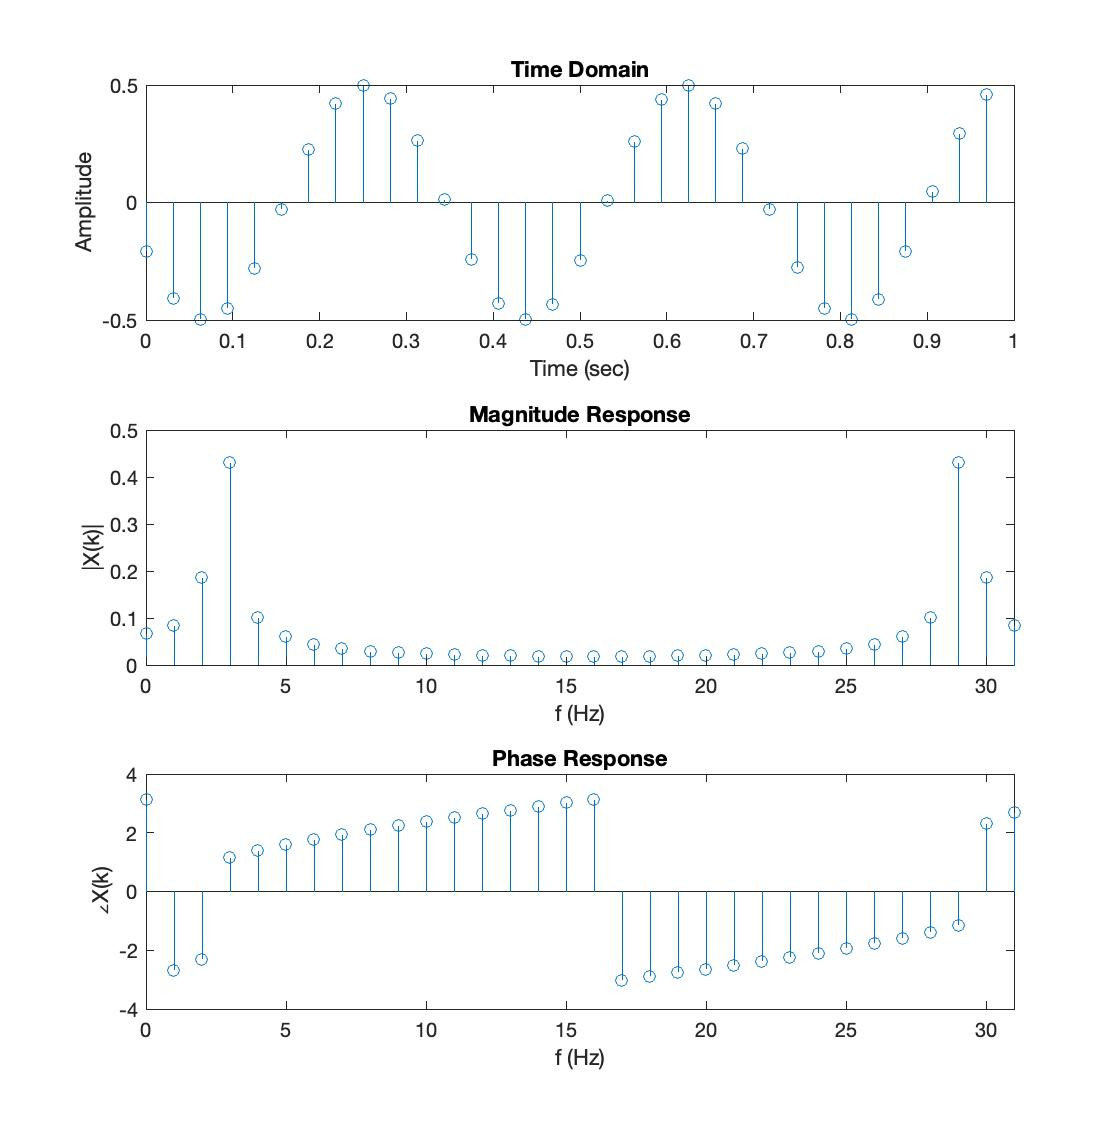
\includegraphics[scale = 0.3]{aperiodic.jpg}
	\end{center}
\end{figure}

Plotted in Figure \ref{fig:aperiodicGraph} is the magnitude and phase spectra of the original signal as well as its time 
domain representation.  Notice that the time domain clearly shows that $x[n]$ completes
two full cycles \textbf{plus} some fractional number of cycles.  After computing the DFT of $x[n]$, Figure 
\ref{fig:aperiodicGraph} shows the magnitude and phase spectra.
The magnitude spectrum was calculated by taking the magnitude of each complex number.  
If we look at the graph, we can see two peaks roughly between 2Hz and 3Hz
and between 29Hz and 30Hz.  We can also see the symmetry between the two halves if we split the magnitude spectrum
down the middle.  We can see that every frequency bin has some magnitude in it which might suggest that our original
signal was composed of 32 sinusoids of varying amplitudes.  But we know that is not the case.  There is just one at
2.7Hz.  We can, however, see ``activity" at 2.7Hz in the magnitude spectrum due to the vertical peak.  The other peak
is simply the mirror image of 2.7Hz above the Nyquist frequency.  We saw this symmetry occurred even with periodic
sinusoids.  So many of the same instincts that we derived in the context or periodic $x[n]$ hold true with aperiodic 
$x[n]$. 

How do we account though for positive magnitudes in all the bins?  This is a phenomenon called \textbf{spectral leakage}.  
We will always see peaks in the magnitude spectrum at the frequencies of $x[n]$ provided those frequencies have
sufficient amplitude.  Notice though that each frequency bin registers some level of magnitude.  Farther away from the 
peak, the magnitudes decrease but are still non-zero.  This is called ``spectral leakage".  It is important to understand
that we are not seeing multiple frequencies.  Rather we are seeing the effect of how one aperiodic component of $x[n]$
spreads out to all frequency bins.   

Can we recover the original amplitude of 0.5 from the magnitude spectrum?  The answer, in short, is no.  For one, we
would need to guess about where the apex of the peak was.  The peak is always centered at the frequency of each
component of $x[n]$.  It is hard to tell based on the magnitude spectrum though where exactly that is.  We can use
a process called interpolation to estimate the peak.  Even so, each frequency component of $x[n]$ spreads to each
adjacent bin.  Therefore, even if we could determine the peak, the magnitude at that location could be the product
of the spread of several different peaks.  Therefore, it will be impossible to reconstruct the original amplitude.  
Nevertheless we can get a good sense of the relative strength of each component.  Higher peaks represent stronger
frequency components; lower peaks represent weaker frequency components.

How can we interpret the phase spectrum?  Again we see a sudden change around 2Hz.  The phase spectrum shifts
drastically at the location moving from negative to positive.  It is hard though to see any relationship between the phase spectrum of $x[n]$ around 2.7Hz and the original phase.  In 
general, the phase spectrum of the DFT is more abstruse and difficult to parse.  Sometimes sudden shifts in the
phase spectrum are the result of the periodic nature of sinusoids.  Phases outside the range $+\pi$ to $-\pi$ get
wrapped back down to that range.  This can cause abrupt shifts in the phase spectrum.  We will not be spending
much time examining the phase spectrum as it usually is less important for musical applications. We shall see soon
though that there is a better way to interpret the phase spectrum.

\subsection*{The Periodicity of the DFT}

We have seen how the DFT responds to periodic and aperiodic sinusoids.  In this section, I would like to offer 
another perspective on the DFT.  We have learned that the DFT can accurately parse the frequencies of $x[n]$ if
$x[n]$ is periodic along those $N$ samples.  I should also state explicitly that the DFT \textbf{assumes} that
those $N$ samples are from a periodic function regardless of whether they are or not and that those $N$ samples
constitute a period from that periodic signal $x[n]$.  

If we look back at the time
domain representation of Figure \ref{fig:aperiodicGraph}, we can see a plot of the samples from the sinusoid of
2.7Hz.  The DFT assumes those $N$ samples make up one period of the periodic signal $x[n]$.  $x[n]$
is indeed periodic but those $N$ samples are not a period of $x[n]$.  One way to see what the DFT ``sees" is to
simply repeat those $N$ samples and look at the time domain representation of the sound.  The top plot in Figure
\ref{fig:basis} shows a plot of 2.7Hz with a smaller sampling period to highlight the disjointed transition when the samples
repeat.  Importantly, the DFT is parsing the frequencies of \textbf{this} signal and not the smoothly oscillating sinusoid 
from where the samples originated.  Another way, then,
to think about spectral leakage is that it is the distortion of the original waveform that occurs when we fail
to capture a complete period.

\begin{figure}[h]
	\caption{Periodicity of the DFT as shown through the time domain representation in the samples and the cosine basis}
	\label{fig:basis}
	\begin{center}
		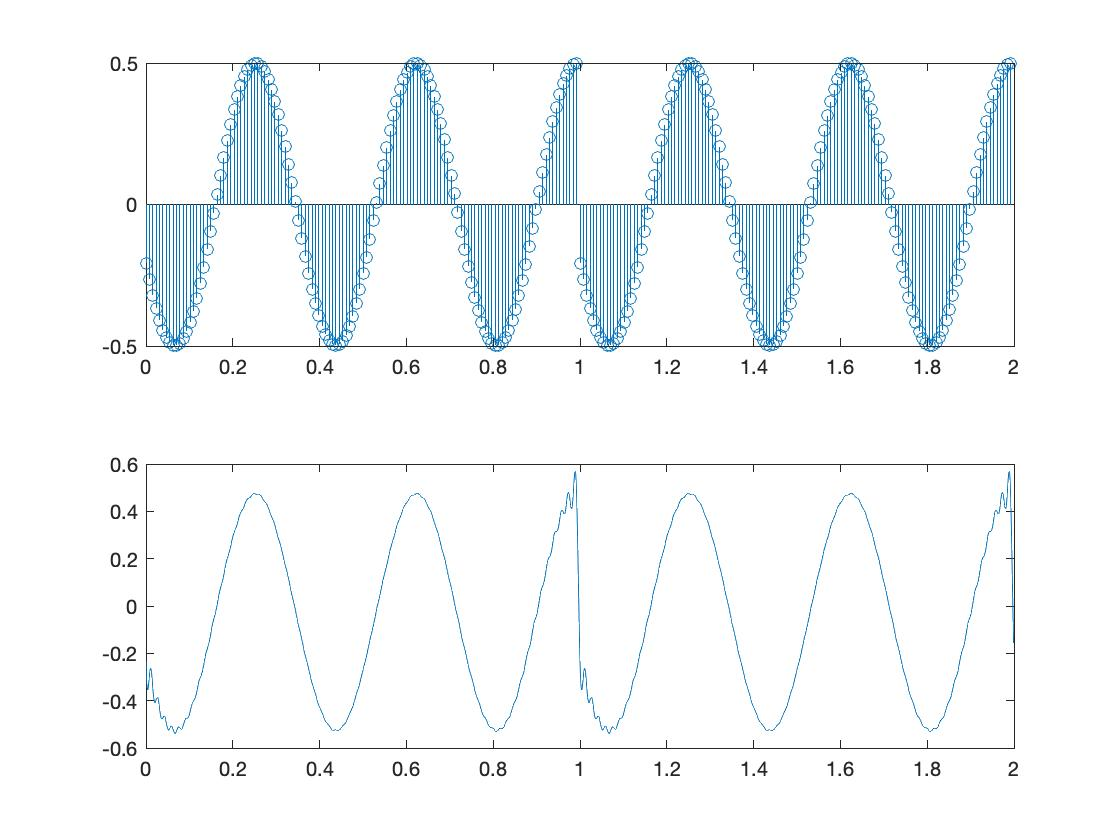
\includegraphics[scale = 0.3]{basis.jpg}
	\end{center}
\end{figure}

Consider again the N aperiodic samples from the sinusoid 2.7Hz. In that example,
we took a slice of $N = 32$ samples from $x[n] = 0.5\cos(2\pi (2.7)Tn + 2)$.  Nevertheless, the DFT still considered those $N$ samples to be periodic.  Again, the top plot in Figure \ref{fig:basis} shows how the DFT perceives the periodicity of that waveform.\footnote{
	Here though we have increased the number of samples and sampling rate 
	($N = 128$ and $f_s = 128$Hz) for higher resolution.
}
Because this distorted signal is periodic, we can represent it using a sum of harmonic sinusoids.  The bottom plot from Figure \ref{fig:basis} shows an approximation of that signal with a sum of harmonic cosine waves.  
How can we determine which cosine waves to sum?  From the DFT, of course!  
\textbf{Another interpretation of the
DFT is that it encodes the information to recreate the N periodic samples using a sum of harmonic cosine waves.}  
The frequencies
of the DFT bins form a harmonic series with a fundamental period equivalent to the time spanned by the $N$ samples.
Therefore, we can use $X_k$ to construct the amplitude and phase of each sinusoid.

The magnitude and phases we calculate for each frequency bin
can be used in conjunction with the frequency of each bin to construct a series of cosines waves that,
when summed, produce the approximation shown in the bottom plot from Figure \ref{fig:basis}.  For example,
the first frequency bin has a frequency of 0 where $X_0 = AN\cos(\phi)$. Remember we are interpreting the $N$ samples
as periodic, therefore we know $X_0 = AN\cos(\phi)$.  For subsequent $X_k$, we can rely on Equation \ref{eq:amplitude} and
\ref{eq:phase} to determine the amplitude and phase of each frequency bin.  For example, the second
 frequency bin has a frequency of 1Hz, a magnitude of 0.0696, and a phase of $-2.6026$.  If we plug those values into
 a cosine wave, we get $0.0696 * \cos(2 * \pi * (1) * t - 2.6026) = 0.0696\cos(2\pi t - 2.6026)$.  We can add this to
 $-0.0261$ to get the first two sinusoidal harmonics.  If we continued in this fashion with every frequency bin
 up to $k = N/2$, the Nyquist frequency, we get the approximation shown in the bottom plot from 
 Figure \ref{fig:basis}.  
 
 	In this interpretation of the DFT, we can see how both the phase and magnitude derive meaning.  We can think
 of the DFT as producing a series of harmonic cosine waves that get their specific parameters from the values in each
frequency bin.  We call these harmonic cosine waves a \textbf{basis}, and we \textbf{project} our original signal
$x[n]$ onto this basis.  This is the geometric interpretation of the DFT.  The terms ``projection" and ``basis" are 
mathematical terms.  One common ``basis" we all know is the coordinate axis system.  It is a space that allows us
to plot any 2D shape.  A series of harmonic cosine waves also form a basis.  It is a basis that allows us to 
plot or describe any periodic signal.  We can think of projection as a means to describe our original signal
 in terms of our basis (i.e., a sum of cosine waves).  But how exactly do we do this projection?  
 With the inner product.  The inner product, with which we started our duscussion of the DFT,
 is a means of projecting a signal onto a different basis such as the frequency domain.  Therefore, another way to
 view the DFT is that it takes a period of $N$ samples and projects them onto a set of harmonic sinusoids that
 approximate the waveform described by those $N$ samples.
